\documentclass{minimal}

\usepackage{pgf}
\usepackage{tikz}
\usepackage[utf8]{inputenc}
\usetikzlibrary{arrows,automata}
\usetikzlibrary{positioning}


\tikzset{
    state/.style={
           rectangle,
           rounded corners,
           draw=black, very thick,
           minimum height=2em,
           inner sep=2pt,
           text centered,
           },
}

\begin{document}

\begin{tikzpicture}[->,>=stealth']

 % Position of QUERY 
 % Use previously defined 'state' as layout (see above)
 % use tabular for content to get columns/rows
 % parbox to limit width of the listing
 \node[state] (QUERY) 
 {\begin{tabular}{l}
  \textbf{Query}\\
  \parbox{4cm}{\begin{itemize}
   \item Start
   \item Parameter $Q$
   \item Zufallszahl aus \mbox{$[0, 2^Q-1]$} in Slotzähler $SC$
  \end{itemize}
  }\\[4em]
  \textbf{QueryAdjust}\\
  \parbox{4cm}{\begin{itemize}
   \item Variiere Q
   \item neue Zufallszahl
  \end{itemize}
  }
 \end{tabular}};
  
 % State: ACK with different content
 \node[state,    	% layout (defined above)
  text width=3cm, 	% max text width
  yshift=2cm, 		% move 2cm in y
  right of=QUERY, 	% Position is to the right of QUERY
  node distance=6.5cm, 	% distance to QUERY
  anchor=center] (ACK) 	% posistion relative to the center of the 'box'
 {%
 \begin{tabular}{l} 	% content
  \textbf{Ack}\\
  \parbox{2.8cm}{Bestätigen mit $RN_{16}$}
 \end{tabular}
 };
 
 % STATE QUERYREP
 \node[state,
  below of=ACK,
  yshift=-2cm,
  anchor=center,
  text width=3cm] (QUERYREP) 
 {%
 \begin{tabular}{l}
  \textbf{QueryRep}\\
  \parbox{2.8cm}{Dekrementiere Slotzähler}
 \end{tabular}
 };

 % STATE EPC
 \node[state,
  right of=ACK,
  node distance=5cm,
  anchor=center] (EPC) 
 {%
 \begin{tabular}{l}
  Antwort: \textbf{EPC}\\
  \parbox{4cm}{Mit nächstem \mbox{\textbf{QueryRep}} als "`inventoried"' markieren.}
 \end{tabular}
 };

 % draw the paths and and print some Text below/above the graph
 \path (QUERY) 	edge[bend left=20]  node[anchor=south,above]
                                    node[anchor=north,below]{$RN_{16}$} (ACK)
 (QUERY)     	edge[bend right=20] node[anchor=south,above]{$SC_n\neq 0$} (QUERYREP)
 (ACK)       	edge                                                     (EPC)
 (EPC)       	edge[bend left]                                          (QUERYREP)
 (QUERYREP)  	edge[loop below]    node[anchor=north,below]{$SC_n\neq 0$} (QUERYREP)
 (QUERYREP)  	edge                node[anchor=left,right]{$SC_n = 0$} (ACK);

\end{tikzpicture}


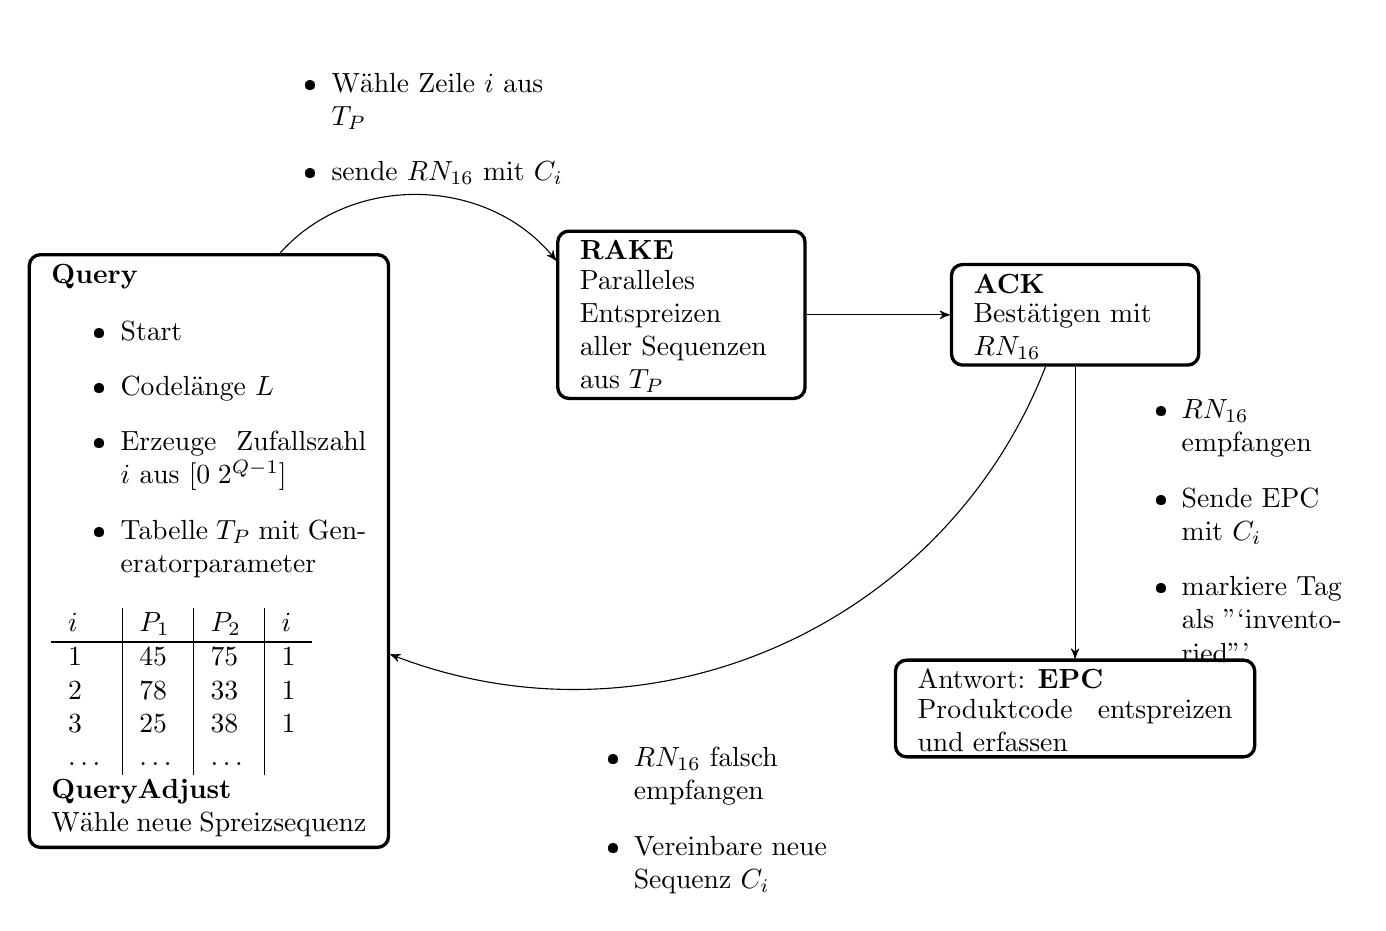
\begin{tikzpicture}[->,>=stealth']

 % First node
 % Use previously defined 'state' as layout (see above)
 % use tabular for content to get columns/rows
 % parbox to limit width of the listing
 \node[state] (QUERY) 
 {\begin{tabular}{l}
  \textbf{Query}\\
  \parbox{4cm}{\begin{itemize}
   \item Start
   \item Codelänge $L$
   \item Erzeuge Zufallszahl $i$ aus $[0 \; 2^{Q-1}]$
   \item Tabelle $T_P$ mit Generatorparameter
  \end{itemize}
  \begin{tabular}{l|l|l|l}
   $i$ & $P_1$ & $P_2$ & $i$ \\\hline
   $1$ & $45$ & $75$ & $1$\\
   $2$ & $78$ & $33$ & $1$\\
   $3$ & $25$ & $38$ & $1$\\
   \ldots & \ldots & \ldots
  \end{tabular}
  }\\[4em]
  \textbf{QueryAdjust}\\
  \parbox{4cm}{Wähle neue Spreizsequenz}
 \end{tabular}};

 % Next node: RAKE
 \node[state,       % layout (defined above)
 node distance=6cm,     % distance to QUERY
 text width=3cm,        % max text width
 right of=QUERY,        % Position is to the right of QUERY
 yshift=+3cm] (RAKE)    % move 3cm in y
 {%                     % posistion relative to the center of the 'box'
 \begin{tabular}{l}     % content
  \textbf{RAKE}\\
  \parbox{2.8cm}{Paralleles Entspreizen aller Sequenzen aus $T_P$}
 \end{tabular}
 };

 % STATE ACK
 \node[state,
 right of=RAKE,
 node distance=5cm,
 text width=3cm] (ACK) 
 {%
 \begin{tabular}{l}
  \textbf{ACK}\\
  \parbox{2.8cm}{Bestätigen mit $RN_{16}$}
 \end{tabular}
 };

 % STATE EPC
 \node[state,
 below of=ACK,
 node distance=5cm] (EPC) 
 {%
 \begin{tabular}{l}
  Antwort: \textbf{EPC}\\
  \parbox{4cm}{Produktcode entspreizen und erfassen}
 \end{tabular}
 };

 % draw the paths and and print some Text below/above the graph
 \path (QUERY) edge[bend left=50]  node[anchor=south,above,text width=4cm]
                   {
                   \begin{itemize}
                    \item Wähle Zeile $i$ aus $T_P$
                    \item sende $RN_{16}$ mit $C_i$
                   \end{itemize}
                   } (RAKE)
 (RAKE) edge                    (ACK)
 (ACK)  edge                    node[anchor=east,right,text width=3cm,xshift=1em]
                  {
                  \begin{itemize}
                   \item $RN_{16}$ empfangen
                   \item Sende EPC mit $C_i$
                   \item markiere Tag als "`inventoried"'
                  \end{itemize}
                  } (EPC)

 (ACK)  edge[bend left=45] node[anchor=north,below,text width=4cm,yshift=-2em,xshift=-2em]
                  {\begin{itemize}
                   \item $RN_{16}$ falsch empfangen
                   \item Vereinbare neue Sequenz $C_i$
                  \end{itemize}
                  } (QUERY)
 ;
\end{tikzpicture}
\end{document}
